


\chapter{Implementing FLIP}
\label{chapter flip impl}

In order to achieve real time simulation, algorithm \ref{algo multiphase flip} needs to be executed at maximum performance. This project approaches this by exploiting the parallel computing power of modern GPUs. This chapter begins by giving a short introduction to GPU computing, and then explains the parallel version of algorithm \ref{algo multiphase flip} designed and implemented in this project. Some special GPU memory access optimizations in the implementation, which considerably boosted the efficiency of the simulation, are also discussed. 

\section{The CUDA Programming Model}

Originally built for graphics applications, GPUs are designed to handle a massive amount of geometries and pixels in parallel, because in graphics applications the computation for different geometries and pixels are largely independent. The ability to do massively parallel computation motivated GPGPU (General Purpose GPU) programming models to arise, which became significantly useful for scientific computing purposes. The software in this project is written using the CUDA programming model, developed by the NVIDIA Corporation.

CUDA employs the executing model known as SIMT (Single Instruction Multiple Thread). In this model, a large amount of GPU threads can be spawned simultaneously, each running the same sequence of code on different sets of data. GPU threads are organized in groups of 32, known as \textit{warps}, and the instructions running on threads of the same warp must be synchronized. However, different warps does not need to remain in sync. When the threads within a warp access the memory, the entire warp can be swapped out, so that a different warp can start executing before the memory access finishes. Using this mechanism, the GPU hides memory access latencies by allowing very fast context switching. As a result, each physical core in the GPU (known as a CUDA core) can simultaneously handle multiple logical threads.

As an example, the GPU used for development of this project is an NVIDIA GTX1060 Mobile, which contains 10 \textit{Streaming Multiprocessors}, each of which consists of 128 CUDA cores. Each streaming multiprocessors can have up to 2048 resident threads, giving a total of 20480 threads that can be simultaneously handled. Even though each GPU thread is not as fast as a CPU thread, the aggregated performance of the CUDA cores can still be many times faster than the CPU.


\begin{figure}[H]
    \centering
    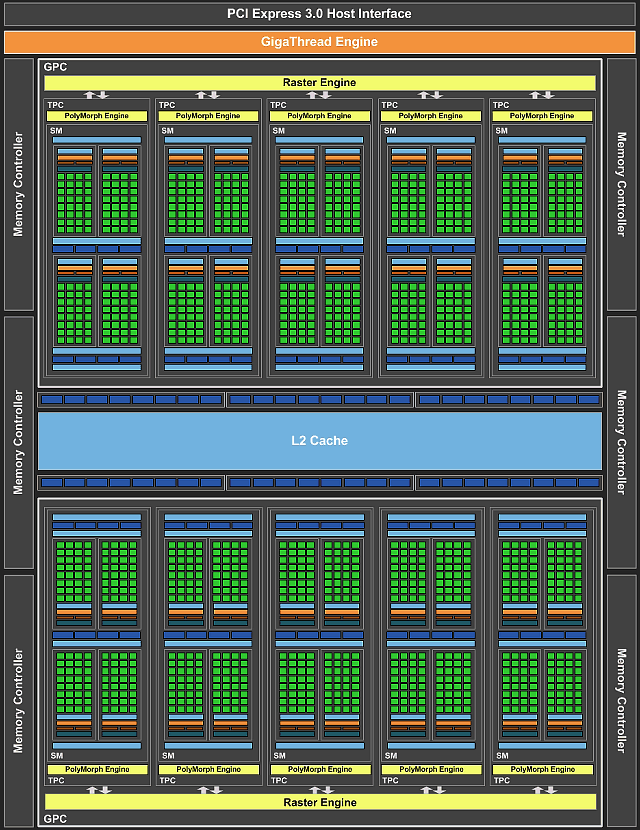
\includegraphics[width=12cm]{gp106}
    \caption{Architecture of a GTX 1060 (GP106), showing its 10 streaming multiprocessors, each containing 128 CUDA cores. Image courtesy to NVIDIA Corporation.}
    \label{figure GTX1060}
\end{figure}



\section{Parallelization}
The pseudocode representation of algorithm \ref{algo multiphase flip} takes a sequential form, so in order to create an efficient CUDA implementation, the challenge remains to parallelize the algorithm.

For certain parts of the algorithm, parallelization is straightforward. Examples include line 2-4 and line 8-9 within the qseudocode. These are all operations performed within a loop body, with the convenient property that, in different loop iterations, the data being operated on are completely different, and does not depend on previous iterations. This means it is safe to use parallel threads instead of actual loops to perform these operations. Similarly, the velocity field updates in line 11 and 13 are also easy to parallelize, with each thread operating on one grid cell of the discretized velocity field. 

The rest of the algorithm, line 7, 12 and 14, requires much more attention. Line 7 performs a task called \textit{spatial indexing}: associating each grid cell with all the particles that are within radius $\triangle x$ at each time step. A naive implementation would require a linear search on all particles, and this has to be performed for all grid cells, which is intolerable because the simulation could involve up to around 1,000,000 particles and 100,000 grid cells. In line 12 and 14, a linear equation needs to be solved, where there's an unknown for each fluid cell. As a result, the total amount of unknowns is in the order of 100,000. A naive linear solver have a $O(N^3)$ complexity, which is also too costly. Each of these operations, indexing 1,000,000 million particles and solving linear equations with 100,000 unknowns, needs to be performed at least around 20 times per second, if the simulation is to be performed in real time. This section will focus on how this is made possible in this project.

\subsection{Spatial Indexing}
\label{subsection spatial indexing}
With $\triangle x$ being the edge length of each cubic grid cell, finding all particles within a radius $\triangle x$ of each cell can be reduced to finding the particles that are \textit{inside} each cell. Then, for a certain cell, it suffices to check all the 27 cells in the neighborhood, because all particles within a radius $\triangle x$ must be contained inside these 27 cells. 


To create an index from each cell to the particles inside the cell, this project uses the parallel algorithm proposed by Green \cite{green2008cuda}. The algorithm proceeds in the following steps:

\begin{figure}[p]
    \begin{minipage}[t]{.65\linewidth}
        \vspace{0pt}
        \centering
        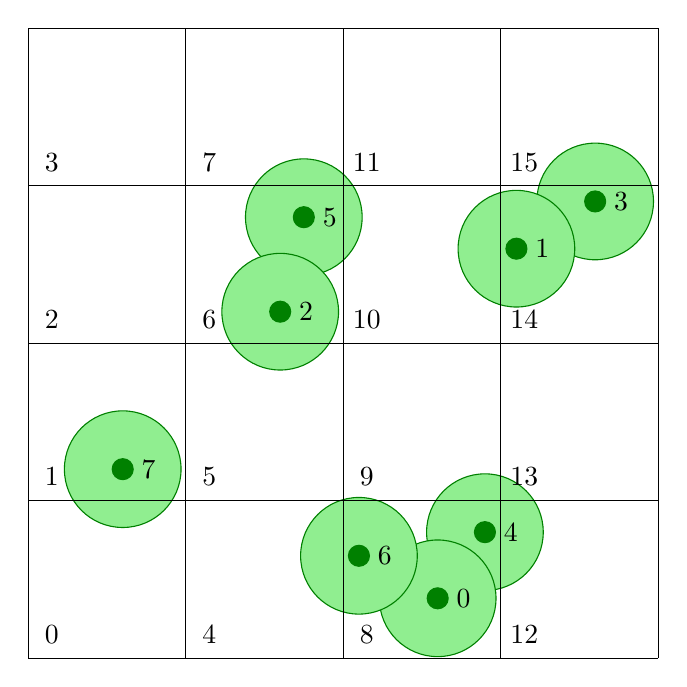
\begin{tikzpicture} 
            \pgfmathsetmacro\dx{2};
            \pgfmathsetmacro\radius{\dx / 2.7};
            \pgfmathsetmacro\centerRadius{\dx / 15};

            \pgfmathsetmacro\x{0.6*\dx};
            \pgfmathsetmacro\y{1.2*\dx};
            \filldraw[draw=Green,fill=LightGreen] (\x,\y) circle (\radius);
            \filldraw[draw=Green,fill=Green] (\x,\y) circle (\centerRadius) node[right]{~7};

            \pgfmathsetmacro\x{1.75*\dx};
            \pgfmathsetmacro\y{2.8*\dx};
            \filldraw[draw=Green,fill=LightGreen] (\x,\y) circle (\radius);
            \filldraw[draw=Green,fill=Green] (\x,\y) circle (\centerRadius)node[right]{~5};

            \pgfmathsetmacro\x{1.6*\dx};
            \pgfmathsetmacro\y{2.2*\dx};
            \filldraw[draw=Green,fill=LightGreen] (\x,\y) circle (\radius);
            \filldraw[draw=Green,fill=Green] (\x,\y) circle (\centerRadius)node[right]{~2};

            \pgfmathsetmacro\x{2.9*\dx};
            \pgfmathsetmacro\y{0.8*\dx};
            \filldraw[draw=Green,fill=LightGreen] (\x,\y) circle (\radius);
            \filldraw[draw=Green,fill=Green] (\x,\y) circle (\centerRadius)node[right]{~4};

            \pgfmathsetmacro\x{2.6*\dx};
            \pgfmathsetmacro\y{0.38*\dx};
            \filldraw[draw=Green,fill=LightGreen] (\x,\y) circle (\radius);
            \filldraw[draw=Green,fill=Green] (\x,\y) circle (\centerRadius)node[right]{~0};

            \pgfmathsetmacro\x{2.1*\dx};
            \pgfmathsetmacro\y{0.65*\dx};
            \filldraw[draw=Green,fill=LightGreen] (\x,\y) circle (\radius);
            \filldraw[draw=Green,fill=Green] (\x,\y) circle (\centerRadius)node[right]{~6};

            \pgfmathsetmacro\x{3.6*\dx};
            \pgfmathsetmacro\y{2.9*\dx};
            \filldraw[draw=Green,fill=LightGreen] (\x,\y) circle (\radius);
            \filldraw[draw=Green,fill=Green] (\x,\y) circle (\centerRadius)node[right]{~3};

            \pgfmathsetmacro\x{3.1*\dx};
            \pgfmathsetmacro\y{2.6*\dx};
            \filldraw[draw=Green,fill=LightGreen] (\x,\y) circle (\radius);
            \filldraw[draw=Green,fill=Green] (\x,\y) circle (\centerRadius)node[right]{~1};

            

            \foreach \x in {0,1,2,3}{
                \foreach \y in {0,1,2,3}{  
                    \draw (\x*\dx,\y*\dx) -- (\x*\dx+\dx,\y*\dx);
                    \draw (\x*\dx,\y*\dx) -- (\x*\dx,\y*\dx+\dx);
                    \draw (\x*\dx+\dx,\y*\dx) -- (\x*\dx+\dx,\y*\dx+\dx);
                    \draw (\x*\dx,\y*\dx+\dx) -- (\x*\dx+\dx,\y*\dx+\dx);
                    \pgfmathtruncatemacro\result{\x*4 + \y};
                    \node at (\x*\dx+0.3,\y*\dx+0.3) {\result};
                }
            }

            
            
        \end{tikzpicture}
        \subcaption{The indices and positions of the particles in the grid before spatial indexing.}
        

    \end{minipage}%
    \begin{minipage}[t]{.33\linewidth}
        \vspace{0pt}
        \centering
        \begin{tabular}{|c | c |} 
            \hline
            particle & hash \\ [0.5ex] 
            \hline\hline
            0 & 8  \\ 
            \hline
            1 & 14  \\ 
            \hline
            2 & 6  \\ 
            \hline
            3 & 14  \\ 
            \hline
            4 & 8  \\ 
            \hline
            5 & 6  \\ 
            \hline
            6 & 8  \\ 
            \hline
            7 & 1  \\ 
            \hline
            

            
        \end{tabular}
        \subcaption{The array of hashes of particles, computed in step 2.}
    \end{minipage}%

    \hspace{20pt}

    \begin{minipage}[t]{.65\linewidth}
        \vspace{0pt}
        \centering
        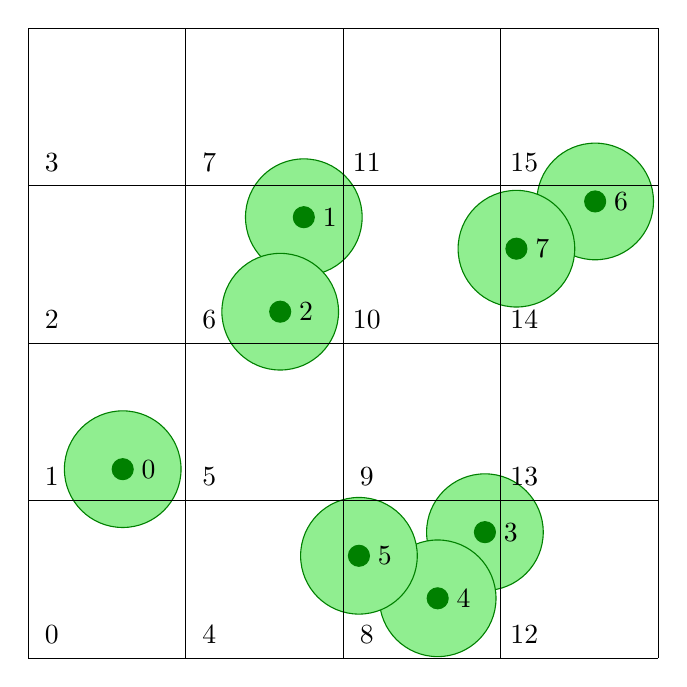
\begin{tikzpicture} 
            \pgfmathsetmacro\dx{2};
            \pgfmathsetmacro\radius{\dx / 2.7};
            \pgfmathsetmacro\centerRadius{\dx / 15};

            \pgfmathsetmacro\x{0.6*\dx};
            \pgfmathsetmacro\y{1.2*\dx};
            \filldraw[draw=Green,fill=LightGreen] (\x,\y) circle (\radius);
            \filldraw[draw=Green,fill=Green] (\x,\y) circle (\centerRadius) node[right]{~0};

            \pgfmathsetmacro\x{1.75*\dx};
            \pgfmathsetmacro\y{2.8*\dx};
            \filldraw[draw=Green,fill=LightGreen] (\x,\y) circle (\radius);
            \filldraw[draw=Green,fill=Green] (\x,\y) circle (\centerRadius)node[right]{~1};

            \pgfmathsetmacro\x{1.6*\dx};
            \pgfmathsetmacro\y{2.2*\dx};
            \filldraw[draw=Green,fill=LightGreen] (\x,\y) circle (\radius);
            \filldraw[draw=Green,fill=Green] (\x,\y) circle (\centerRadius)node[right]{~2};

            \pgfmathsetmacro\x{2.9*\dx};
            \pgfmathsetmacro\y{0.8*\dx};
            \filldraw[draw=Green,fill=LightGreen] (\x,\y) circle (\radius);
            \filldraw[draw=Green,fill=Green] (\x,\y) circle (\centerRadius)node[right]{~3};

            \pgfmathsetmacro\x{2.6*\dx};
            \pgfmathsetmacro\y{0.38*\dx};
            \filldraw[draw=Green,fill=LightGreen] (\x,\y) circle (\radius);
            \filldraw[draw=Green,fill=Green] (\x,\y) circle (\centerRadius)node[right]{~4};

            \pgfmathsetmacro\x{2.1*\dx};
            \pgfmathsetmacro\y{0.65*\dx};
            \filldraw[draw=Green,fill=LightGreen] (\x,\y) circle (\radius);
            \filldraw[draw=Green,fill=Green] (\x,\y) circle (\centerRadius)node[right]{~5};

            \pgfmathsetmacro\x{3.6*\dx};
            \pgfmathsetmacro\y{2.9*\dx};
            \filldraw[draw=Green,fill=LightGreen] (\x,\y) circle (\radius);
            \filldraw[draw=Green,fill=Green] (\x,\y) circle (\centerRadius)node[right]{~6};

            \pgfmathsetmacro\x{3.1*\dx};
            \pgfmathsetmacro\y{2.6*\dx};
            \filldraw[draw=Green,fill=LightGreen] (\x,\y) circle (\radius);
            \filldraw[draw=Green,fill=Green] (\x,\y) circle (\centerRadius)node[right]{~7};

            

            \foreach \x in {0,1,2,3}{
                \foreach \y in {0,1,2,3}{  
                    \draw (\x*\dx,\y*\dx) -- (\x*\dx+\dx,\y*\dx);
                    \draw (\x*\dx,\y*\dx) -- (\x*\dx,\y*\dx+\dx);
                    \draw (\x*\dx+\dx,\y*\dx) -- (\x*\dx+\dx,\y*\dx+\dx);
                    \draw (\x*\dx,\y*\dx+\dx) -- (\x*\dx+\dx,\y*\dx+\dx);
                    \pgfmathtruncatemacro\result{\x*4 + \y};
                    \node at (\x*\dx+0.3,\y*\dx+0.3) {\result};
                }
            }

            

            
        \end{tikzpicture}
        \subcaption{The indices and positions of the particles, after they are sorted according to their hashes, in step 3.}
    \end{minipage}%
    \begin{minipage}[t]{.43\linewidth}
        \vspace{0pt}
        \centering
        \begin{tabular}{|c | c | c|} 
            \hline
            cell & $cellStart$ & $cellEnd$ \\ [0.5ex] 
            \hline\hline
            0 & ~ & ~ \\ 
            \hline
            1 & 0 & 0 \\ 
            \hline
            2 & ~ & ~ \\ 
            \hline
            3 & ~ & ~ \\ 
            \hline
            4 & ~ & ~ \\ 
            \hline
            5 & ~ & ~ \\ 
            \hline
            6 & 1 & 2 \\ 
            \hline
            7 & ~ & ~ \\ 
            \hline
            8 & 3 & 5 \\ 
            \hline
            9 & ~ & ~ \\ 
            \hline
            10 & ~ & ~ \\ 
            \hline
            11 & ~ & ~ \\ 
            \hline
            12 & ~ & ~ \\ 
            \hline
            13 & ~ & ~ \\ 
            \hline
            14 & 6 & 7 \\ 
            \hline
            15 & ~ & ~ \\ 
            \hline

            
        \end{tabular}
        \subcaption{The final result of spatial indexing, represented as the $cellStart$ and $cellEnd$ array.}
    \end{minipage}%

    \caption{Example of spatial indexing in 2D}
    \label{figure spatial indexing}
\end{figure}


\begin{enumerate}
    \item Decide on a hash function for 3D grid coordinates. For example, in an $N*N*N$ grid, the hash of the coordinate $(x,y,z)$ can be $xN^2+yN+z$, which fully avoids hash collision.
    
    \item Create an array of hashes for particles. For each particle, use its physical position to compute the cell that it is in, and compute the hash of that cell as the hash of the particle. Store the hashes of all particles in this array. Since these steps is independent for each particle, it can be efficiently parallelized.
    
    \item Sort this array of particle hashes, and sort the array of particles into the same order. 
    
    \item Create two arrays $cellStart$ and $cellEnd$, which denote, for each cell, the first and the last particle inside the cell. To compute elements of these arrays, for the $i$th particle, use the hash array to check if the $i-1$th particle is in the same cell, if not, the $cellStart$ of this cell should be $i$. Similarly, if the $i+1$th particle is not in the same cell, the $cellEnd$ of this cell should be $i$. This can also be done for all particles in parallel.
    
\end{enumerate}
Having created the $cellStart$ and $cellEnd$ arrays, for each cell, the particles inside it is them simply the particles with index $\geq cellStart$ and $\leq cellEnd$. A 2D example of this procedure is illustrated in figure \ref{figure spatial indexing}.

With all other steps being completely parallelizable, the only complicated step is sorting the array of particle hashes. The implementation of this project uses the thoroughly optimized sorting library provided with the CUDA API. The resulting cost of the spatial indexing is almost negligible compared to other tasks, such as solving systems of linear equations.



\subsection{Jacobi Linear Solver}
The two linear systems to be solved in each simulation step, the Poisson pressure equation and the diffusion equation, both have the special property of being \textit{symmetric positive-definite}. Many advanced approaches have been proposed on how to solve these types of matrices, such as ICPCG \cite{bridson2015fluid} and \textit{Geometric Multigrid}\cite{chentanez2011real}. This project chooses to implement a simpler algorithm, called the Jacobi solver. Though not as fast as the most advanced methods, its efficiency and accuracy is found to be sufficient for the real time simulations in this project.

In the Jacobi Solver, given a system of linear equations written in matrix form:
$$
A\textbf{x}=\textbf{b}
$$
the matrix $A$ is decomposed into $D+C$, where $D$ is a diagonal matrix, and $C$ has only $0$s on the diagonal:
$$
(D+C)\textbf{x}=\textbf{b}
$$
The system is then rewritten as 
$$
D\textbf{x}=\textbf{b} - C\textbf{x}
$$
Thus,
$$
\textbf{x}=D^{-1}(\textbf{b} - C\textbf{x})
$$
which motives an iterative scheme: begin with an initial guess $\textbf{x}_0$, and then iteratively compute
\begin{equation}
    \textbf{x}_{i+1} = D^{-1}(\textbf{b} - C\textbf{x}_{i})
    \label{eqn jacobi}
\end{equation}
For a certain amount of iterations. The computation of this formula between different unknowns are completely independent. Therefore, by designating a CUDA thread for each unknown $x$ (and thus, for each cell), the Jacobi iteration step is completely parallelized.

Additionally, by observing the pressure equation \ref{eqn poisson pressure} and the diffusion equation \ref{eqn diffusion}, a further simplification can be made, because the matrix $C$ corresponding to these equations has some convenient properties. For the unknown $x$ corresponding to each cell, the row of $C$ corresponding to that cell only has non-zero entries for immediately adjacent cells. Consequently, for each cell, the computation of formula \ref{eqn jacobi} only requires sampling the $x$ at adjacent cells. This leads to a very efficient parallel implementation of the Jacobi iteration:


\begin{algorithm}[H]
    \label{algo jacobi}
    \SetAlgoLined
    %\For{some amount of iterations}{
        \ForEach{grid cell \textbf{in parallel}}{
            Let the coordinate of the cell be $(i,j,k)$\;
            Retrieve the scalars $D_{(i,j,k)}$ and $b_{(i,j,k)}$\;
            $neighborValues := 0$\;
            Sample the left cell: $neighborValues \mbox{ += } C_{(i-1,j,k)}~x_{(i-1,j,k)}$\;
            Sample the right cell: $neighborValues \mbox{ += } C_{(i+1,j,k)}~x_{(i+1,j,k)}$\;
            Sample the lower cell: $neighborValues \mbox{ += } C_{(i,j-1,k)}~x_{(i,j-1,k)}$\;
            Sample the upper cell: $neighborValues \mbox{ += } C_{(i,j+1,k)}~x_{(i,j+1,k)}$\;
            Sample the back cell: $neighborValues \mbox{ += } C_{(i,j,k-1)}~x_{(i,j,k-1)}$\;
            Sample the front cell: $neighborValues \mbox{ += } C_{(i,j,k+1)}~x_{(i,j,k+1)}$\;
            Update $x_{(i,j,k)}:= (b_{(i,j,k)} - neighborValues) / D_{(i,j,k)} $ 
        }
    %}
    
    
    \caption{Parallel Jacobi Iteration}
\end{algorithm}

Using the parallel spatial indexing algorithm and the Jacobi linear solver, the updated FLIP algorithm is now described as:


\gapM

\begin{algorithm}[H]
    \label{algo multiphase flip parallel}

    \SetAlgoLined
    \tcp{At time step [n+1]}
    \ForEach{particle $p$ \textbf{in parallel}}{
        $\u_p := \u_p + \u_{[n]}(\textbf{x}_p) - \u_{[n-1]}(\textbf{x}_p)$ \;
        $\bm{\alpha}_p := \bm{\alpha}_p + \bm{\alpha}_{[n]}(\textbf{x}_p) - \bm{\alpha}_{[n-1]}(\textbf{x}_p)$ \;
        Move $p$ inside the velocity field using Runge-Kutta\;
    }
    Perform spatial indexing\;
    \ForEach{grid cell at location $(x,y,z)$\textbf{in parallel}}{
        Compute $\u_{[n+1]}^{advected}$, as an interpolation of the $\u_p$ of nearby particles\;
        Compute $\bm{\alpha}_{[n+1]}^{advected}$, as an interpolation of the $\bm{\alpha} _p$ of nearby particles\;
    }
    \ForEach{grid cell at location $(x,y,z)$\textbf{in parallel}}{
        Apply external forces at the cell: $\u_{[n+1]}^{compressible} =  FixSolidBoundary(\u_{[n+1]}^{advected} + \triangle t \textbf{g})$\;
    }
    Using Jacobi, solve the Poisson pressure equation to obtain pressure $p$\;
    \ForEach{grid cell at location $(x,y,z)$\textbf{in parallel}}{
        Compute The new velocity field at the cell: $\u_{[n+1]} = \u_{[n+1]}^{compressible} - \triangle t \dfrac{\nabla p}{\rho}$\;
    }
    Using Jacobi, solve the diffusion equation to obtain $\bm{\alpha}_{[n+1]}$.

    \caption{Parallel multiphase phase fluid FLIP simulation step}

\end{algorithm}

\gapM

This parallel formulation of the multiphase FLIP algorithm is now ready to be implemented in CUDA.

\section{Optimizing Grid Access}
While writing the CUDA code for algorithm \ref{algo multiphase flip parallel}, many optimizations are still possible. This section describes one of the most effective optimizations that was made in this project, which is to use a special type of GPU memory, called the $texture$ memory, for storing the discrete grids.

The key observation behind this optimization is that, algorithm \ref{algo multiphase flip parallel} very often performs the operation of accessing the values stored in multiple adjacent grid cells. This happens during advection, in line 2-4, where the velocity field $\textbf{\u}$ and concentration field $\bm{\alpha}$ is sampled at the locations of particles, and thus an interpolation of all nearby MAC sample points is required. This also occurs at line 14 and 18, inside the Jacobi solver. As presented in algorithm \ref{algo jacobi}, in each Jacobi iteration, the thread for each cell samples the values of its 6 adjacent cells. The advection and Jacobi solver are in fact the most costly steps in the simulation, which hints that if it's possible to speed up the access of multiple adjacent grid cells, the performance of the entire algorithm could be noticeably improved.

This memory access pattern as described exhibits \textit{spatial locality}. However, this is not in the sense of the normal 1D address space locality often discussed in the context of CPU programming, but rather a locality in the 3D space. Fortunately, this specific pattern is in fact quite common in traditional computer graphics applications, where operations such as image filtering are constantly performed. GPUs are thus equipped with a special type of memory, called the $texture$ memory, which accelerates these operations. A texture memory maps the 3D grid onto a type of \textit{space filling curve}, where adjacent points in the 3D space often correspond to adjacent points on the curve. A 2D example of such a curve is:

\begin{figure}[H]
    \centering
        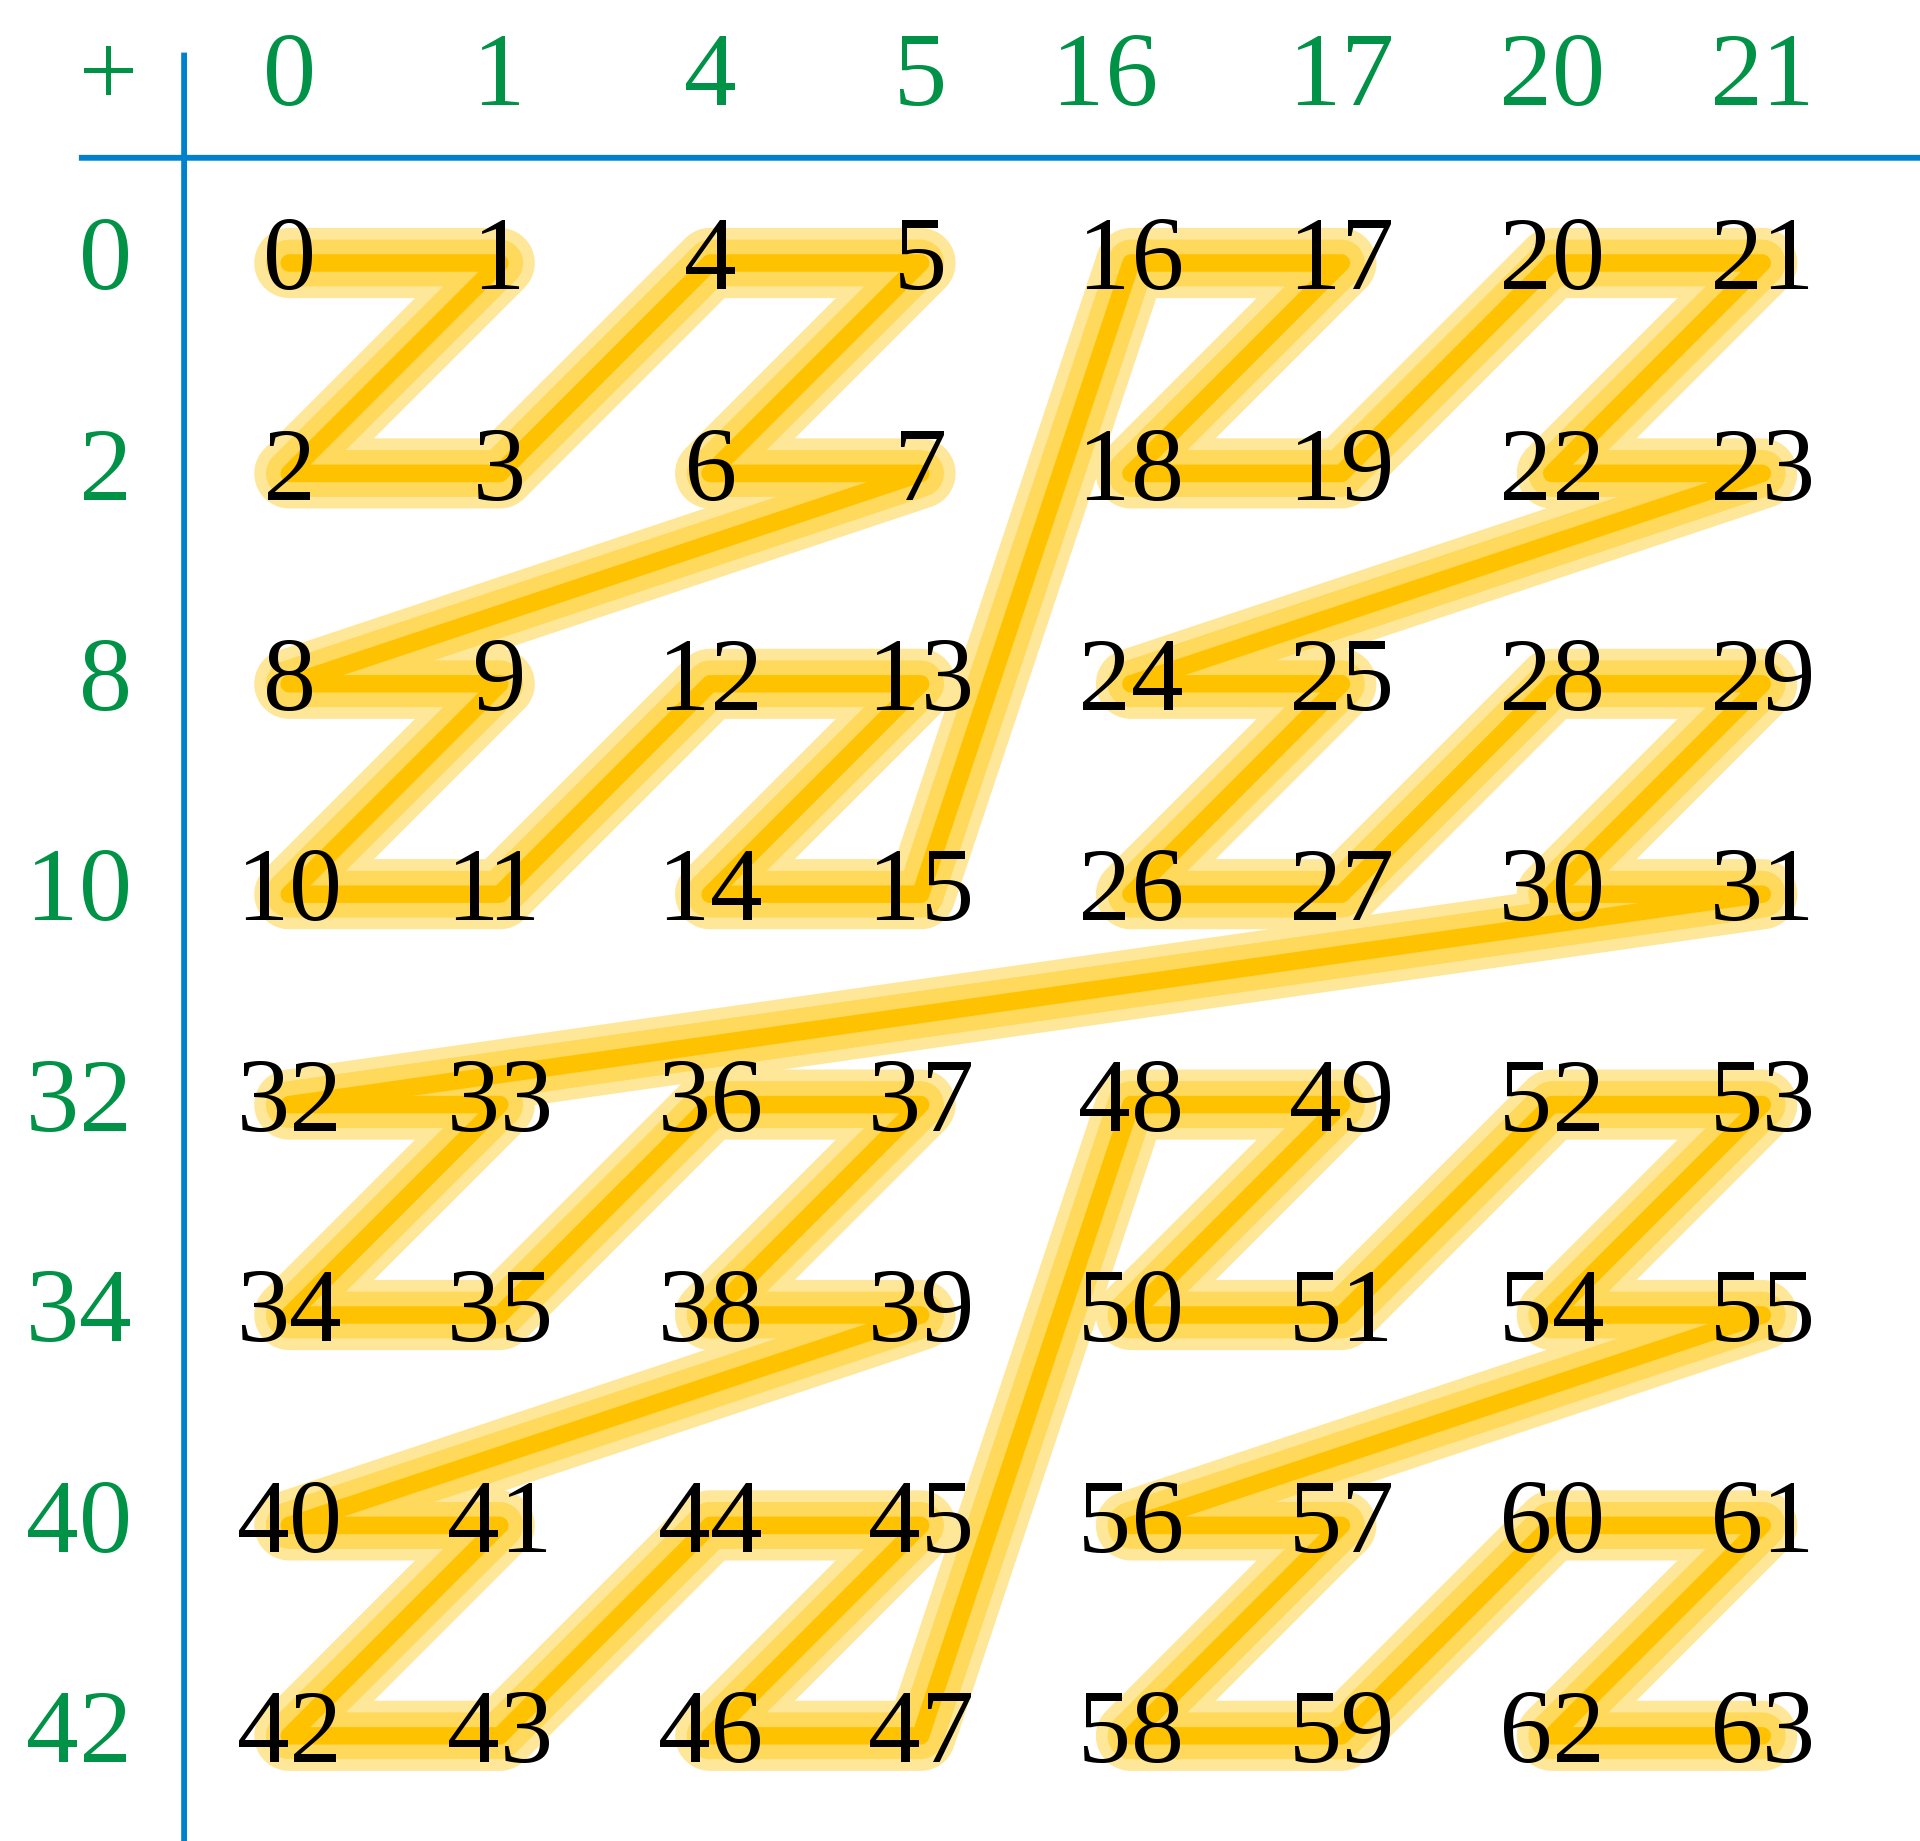
\includegraphics[width=9cm]{curve.png}
    \caption{A Z-order curve. Image courtesy to Wikipedia}
    \label{}
\end{figure}

Using a space filling curve, the texture memory convert the desired 2D/3D spatial locality into 1D locality, which allows the memory access to be more cache friendly. With all the grids stored in textures, the performance of the implementation saw an improvement of 10\% to 20\%.


